\documentclass{article}

% if you need to pass options to natbib, use, e.g.:
% \PassOptionsToPackage{numbers, compress}{natbib}
% before loading nips_2017
%
% to avoid loading the natbib package, add option nonatbib:
% \usepackage[nonatbib]{nips_2017}

\usepackage[final]{nips_2017}

% to compile a camera-ready version, add the [final] option, e.g.:
% \usepackage[final]{nips_2017}

\usepackage{multirow}
\usepackage[utf8]{inputenc} % allow utf-8 input
\usepackage[T1]{fontenc}    % use 8-bit T1 fonts
\usepackage{hyperref}       % hyperlinks
\usepackage{url}            % simple URL typesetting
\usepackage{booktabs}       % professional-quality tables
\usepackage{amsfonts}       % blackboard math symbols
\usepackage{nicefrac}       % compact symbols for 1/2, etc.
\usepackage{microtype}      % microtypography
\usepackage{graphicx}
\graphicspath{ {images/} }

\title{Nerual Phytolith Classifier}

% The \author macro works with any number of authors. There are two
% commands used to separate the names and addresses of multiple
% authors: \And and \AND.
%
% Using \And between authors leaves it to LaTeX to determine where to
% break the lines. Using \AND forces a line break at that point. So,
% if LaTeX puts 3 of 4 authors names on the first line, and the last
% on the second line, try using \AND instead of \And before the third
% author name.

\author{
  James Noeckel, Chenglong Wang\\
  University of Washington
}

\begin{document}
% \nipsfinalcopy is no longer used

\maketitle

\begin{abstract}
  We study the classification problem of phytoliths using stacks of images generated by scanning confocal microscopy. In this report, we present our methods of data preprocessing and dataset augmentation, as well as the accuracy of various models when used as classifiers. Due to the small volume of training data, we avoid using complex models, comparing the accuracy of a linear classifier, a neural network with one hidden fully-connected layer, a neural network with one hidden convolutional layer, and a neural network with two convolutional layers and three fully-connected layers. Additionally, we supervise the classifiers on all three labels (sub-family, tribe, and genus) during training, and additional training data is generated from existing data subjected to random transformations. The results show high performance in differentiating sub-families, and lower performance at the lower rungs of the hierarchy, where some labels have but one example. The single convolutional network performing best on genus and the two-convolutional and three-fully-connected network performing best on sub-family and tribe. The small amount of data makes interpreting test performance difficult, and our tree-based supervision or dataset augmentation do not have consistent effects on accuracy.
\end{abstract}

\section{Introduction}


Phytoliths are microscopic formations of silica found in plant tissues. Their persistence, along with the variation in their shapes and sizes make them particularly useful in archaeological and paleoenvironmental research. Consequently, there is interest in automatically classifying phytoliths from images. Phytolith formations are divided into sub-families, which are in turn divided into tribes, which consist of individual genera.

While there exists a variety of practical image classifiers, the problem for classifying confocal micrographs presents a number of challenges. First, many real world objects, such as phytolith structures or medical scans, are represented in the form of 3D volumes. Instead of directly flattening 2D image stacks into a single image before feeding into a neural network, prior work shows that incorporating 3D structures in image embedding can significantly improve classification results.  In our case, there clearly exist structures that are most prevalent at specific depths, so that aggregating the layers seems like a poor choice. We therefore maintain three-dimensional images in the hopes that our classifiers can learn more meaningful features.

The dataset we used was fairly small (883 image stacks) for training and testing, given that this is an image classification problem. We made some attempts to rectify this using synthetic data samples generated from existing ones, by applying random rotations and scales. Also to aid in classification, we supervised the training using all of the hierarchical class labels together. We conducted a set of experiments using a linear classifier as a baseline, together with several neural net architectures, testing their performance on the dataset when classifying genus, tribe, and sub-family. Our results yield about 60\% accuracy on genus, the lowest level of classification, and about 95\% accuracy at differentiating between the two sub-families.

\section{Problem Description}

The raw data that we are considering for phytolith classification consists of image stacks from confocal micrographs of individual specimen. The images have varying resolution, number of slices, average intensity levels and apparent lighting conditions. Considered as a whole, these image stacks encode a three-dimensional representation of the organisms. However, because each pixel is the result of focusing a cone of light at a particular point in the volume, each slice contains out-of-focus features from every other slice. This makes reconstructing an actual three-dimensional form or surface from the content of the 2D image slices is nontrivial.

The labels are hierarchical, consisting of subfamilies, tribes, and finally the species. All in all, there are 889 data points with around 20 examples per species. Although the data is incredibly high dimensional (in the tens of millions of dimensions) due to being volumetric, there are relatively few examples from which to learn. It is for this reason that we attempt to learn from features that may be present in the volumetric representation of the confocal micrograph, whether or not it corresponds well to the original geometry, in order to train a classifier to predict class labels from image stacks.

\begin{figure}
	\centering
		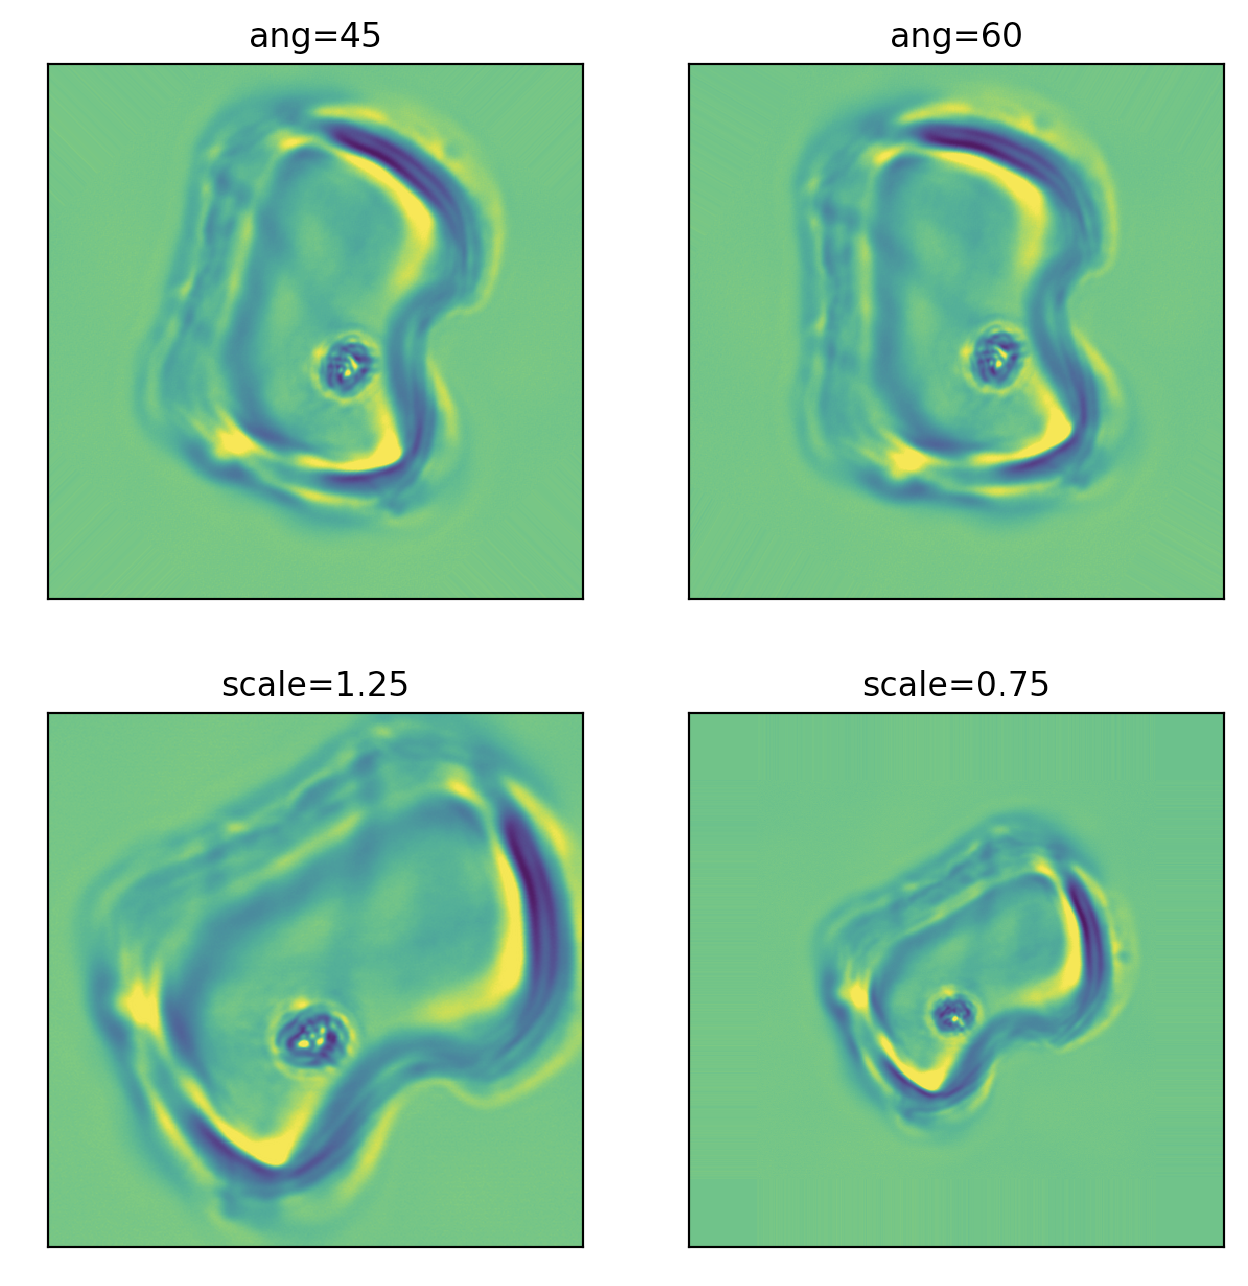
\includegraphics[width=0.5\textwidth]{rotations}
	\caption{Rotated and scaled data generated from a data sample}
	\label{fig:rotated}
\end{figure}

\section{Data Augmentation}

As mentioned, the dataset only contains 889 data samples, resulting in as little as one example in several classes. This motivated us to augment the dataset with random numbers of randomly rotated and scaled variants of each sample in order to provide the classifiers with different vector representations of semantically identical samples. The specific method used to transform the data was cubic spline interpolation, with missing pixels/voxels filled in with using nearest neighbor sampling. Rotations were only with respect to the depth axis, since the optics of a confocal microscope creates highly directional artifacts that would not represent physically correct data at arbitrary orientations. Scales were uniform in all three dimensions in the interest of preserving proportional distances of 3D features. See Figure \ref{fig:rotated} for an example of our synthetic data.


\section{Model Choice}

We experiment with four simple models: linear classifier (LinearModel), a neural network with one hidden layer (FC), a neural network with one convolution layer (Conv) and one network with both convolution layer and a hidden layer (ConvFC). We choose shallow neural models due to the fact that we have a very small training dataset (deep networks would overfit).

In this section, we use ${X}$ and ${y}$ to refer to our training input and output, where each ${x}_i^T\in {X}$ is a vector representing a image and each ${y_i}$ is the label of that image (a 3 dimension array containing genus, tribe and genus information for every image). We use ${p}$ to represent predictions made by our classifier. 


\paragraph{Model}

Each model takes the image vector representation $X$ as input and output the image feature (denoted as $\mathit{outs}$) as a vector of shape $N\times (|F| + |T| + |G|)$ ($|F|, |T|, |G|$ refers to the number of subfamilies, the number of tribes and the number of genus). Concrete model specifications are shown below. Besides, between non-linear layers, we use batch normalization to reduce over-fitting.


\begin{itemize}
	\item (\emph{LinearModel}) $\mathit{outs} = {X} {W} + {b}$
	\item (\emph{FC}) $\mathit{outs} = \mathit{relu}({X} {W}_1 + b_1)\cdot W_2 + b_2$
	\item (\emph{Conv}) $\mathit{outs} = \mathit{maxpool}(\mathit{conv}({X}), d_{\mathit{pool}})\cdot W_2 + b_2$
	\item (\emph{ConvFC}) $\mathit{outs} = \mathit{relu}(\mathit{maxpool}(\mathit{conv}({X}), d_{\mathit{pool}})\cdot W_1 + b_1)\cdot W_2 + b_2$

\end{itemize}

To train these models, we supervise the model on all attributes of the image. Given the output from the model, we first calculate the image's distributions over subfamily, tribe and genus using the softmax function ($t_1, t_2, t_3$ below).

\[
\begin{array}{l}
t_1 = \mathit{softmax}(\mathit{outs}[0:|F|])\\
t_2 = \mathit{softmax}(\mathit{outs}[|F|: |F| + |T|])\\
t_3 = \mathit{softmax}(\mathit{outs}[|F| + |T|:|F| + |T| + |G|])
\end{array}
\]

In training, the loss function is the sum of the cross entropy loss over all three attributes. 
$$L = l_{\mathit{subfamily}} * log(t_1) + l_{\mathit{tribe}} * log(t_2) +  l_{\mathit{genus}} * log(t_3)$$

We optimize the loss with momentum based stochastic gradient descent algorithm.


\section{Experiment}

We run experiments on a singe GPU machine to study the effect of tree based prediction algorithm together as well as the data augmentation scheme. First, we split the data set into 7:1:2 training, dev, test sets, and the splits are uniform among genus, this is intended to avoid having classes that only appear in dev or test set but not in training set.

We conduct a random parameter search process to tune hyper-parameters, and evaluate models with best dev set performance on the test set to report our experiment result. (Table~\ref{t1}) 

After tuning, we find that using images with $32$ stacks of images with size $64\times64$, with the hidden layer feature size $500$, $15$ convolution filters with kernel size $5$ performs best for all models. 

\begin{table}[h]
\centering
\begin{tabular}{ |c|c|c|c|c|c|c|c|c| } 
\hline  
& \multicolumn{2}{|c|}{TP and DA} & \multicolumn{2}{|c|}{TP only} & \multicolumn{2}{|c|}{DA only} & \multicolumn{2}{|c|}{None}\\\cline{2-9}  
 			& Dev    & Test   & Dev    & Test   & Dev    & Test   & Dev    & Test \\\hline\hline 
LinearModel & 42.0\% & 51.0\% & 53.4\% & 41.7\% & 50.0\% & 44.6\% & 54.5\% & 55.4\%\\ 
FC 		 	& 51.1\% & 50.3\% & 62.5\% & 52.9\% & 54.5\% & 49.0\% & 55.7\% & 57.3\%\\ 
Conv 		& 58.0\% & 61.8\% & 62.5\% & 61.8\% & 58.0\% & 51.0\% & 58.0\% & 63.0\%\\
ConvFC 	 	& 58.0\% & 56.1\% & 61.4\% & 58.0\% & 56.8\% & 54.8\% & 55.7\% & 60.5\%\\
\hline
\end{tabular}
\caption{Model accuracies with/without tree prediction (TP) or data augmentation (DA) }
\label{t1}
\end{table}

\paragraph{Discovery} While we expect tree prediction to improve genus prediction at the same time (since it allows the model to learn relationship among images within the same subfamily or class), there is no direct evidence that tree prediction can improve genus prediction. Also, augmenting the dataset add some random effects on the model whether and how much does the augmentation improve the model depends on the model. Another factor of the model's behavior on the dataset is that the dev set remains relatively small (with only 82 examples for 49 classes), and tuning the model based on the dev accuracy may be a factor of the model's under performance.

While the model trained with augmented data and tree predictors under-performs the model without either of them, we still present the result of model accuracy on all subfamily, tribe and genus. The result shows that in the case of performing predictions on all attributes at the same time, ConvFC model performs most stable, being able to achieve better result in high level classification goals, while simple Conv model is more specialized in genus prediction. 

\begin{table}[h]
\centering
\begin{tabular}{ |c|c|c|c|c|c|c|c|c| } 
\hline  
       	    &   Dev (genus) &   Test (genus) & Test (tribe) & Test (subfamily)	\\\hline\hline
LinearModel &  	42.0\%    	&  	51.0\%       &    67.5\%  	&  87.9\% 			\\
FC     		&   51.1\%   	&   50.3\%       &    70.1\%    &  89.8\%			\\
Cov    		&   58.0\%   	&   61.8\%       &    75.8\%   	&  94.3\%			\\
ConvFC 		&   58.0\%   	&   56.1\%       &    77.7\%    &  94.9\%			\\\hline
\end{tabular}
\caption{Accuracies for all models training with both tree prediction and data augmentation. }
\label{t2}
\end{table}

\section{Future Work}

From the model design and experiments, we realized that simply augmenting data is far from enough in improving model performance in case of having too few training examples. Thus using transfer learning with deeper model from Cifar-10 or ImageNet can potentially produce better results. Another improvement might be gained from reducing the less meaningful variation in the data by better aligning the images and normalizing the intensity, perhaps using edge detection.

Another consideration is that when we use tree decoders, we didn't restrict types of sub layer images and the network can still produce false genus for the tribe. Thus we consider restricting decoders with the types can potentially result in better result.

\bibliography{milestone}
\bibliographystyle{plain}
\end{document}